\documentclass{article}
%modified code for hyperplane from \url{http://tex.stackexchange.com/q/104529/86}
\usepackage{tikz}
\usepackage{amsmath}
\usepackage{amsfonts}
\usetikzlibrary{%
  decorations.pathreplacing
}

\makeatletter
\tikzset{
  xyz frame/.code n args={3}{%
    \begingroup
    \tikz@scan@one@point\pgfutil@firstofone#1\relax
    \pgf@xa=\pgf@x
    \pgf@ya=\pgf@y
    \tikz@scan@one@point\pgfutil@firstofone#2\relax
    \pgf@xb=\pgf@x
    \pgf@yb=\pgf@y
    \tikz@scan@one@point\pgfutil@firstofone#3\relax
    \edef\tikz@marshall{\noexpand\endgroup\noexpand\pgfsetxvec{\noexpand\pgfpoint{\the\pgf@xa}{\the\pgf@ya}}%
      \noexpand\pgfsetyvec{\noexpand\pgfpoint{\the\pgf@xb}{\the\pgf@yb}}%
      \noexpand\pgfsetzvec{\noexpand\pgfpoint{\the\pgf@x}{\the\pgf@y}}}%
    \tikz@marshall
  },
  on layer/.code={
    \pgfonlayer{#1}\begingroup
    \aftergroup\endpgfonlayer
    \aftergroup\endgroup
  },
}
\makeatother

\pgfdeclarelayer{behind}
\pgfdeclarelayer{in front}
\pgfsetlayers{behind,main,in front}

\begin{document}
\title{Geometrical visualization of the projection of a point onto a hyperplane}
\author{Andreas Orthey}
\date{}
\maketitle

\def\R{\ensuremath{\mathbb{R}}}

\section{Orthogonal Projection}

Given a point $v_i \in \R^N$, the orthogonal projection onto a hyperplane
$H=\{x\in \R^N| a^Tx=b, \|a\|=1\}$ can be obtained in the following way (see
Figure 1): First we observe that the projection has to be along the
direction of the hyperplane normal from $v_i$, i.e. the we will obtain a form of
$v_i' = v_i - \lambda a$, whereby $\lambda$ is the distance of $v_i$ towards the
hyperplane. Since the distance of the hyperplane to the origin along $a$ is
given by $b$, and the distance of $v_i$ to the origin along $a$ is given by
$v_i^Ta$, we obtain the distance $\lambda = v_i^Ta-b$. 

\begin{figure}[h]
\centering
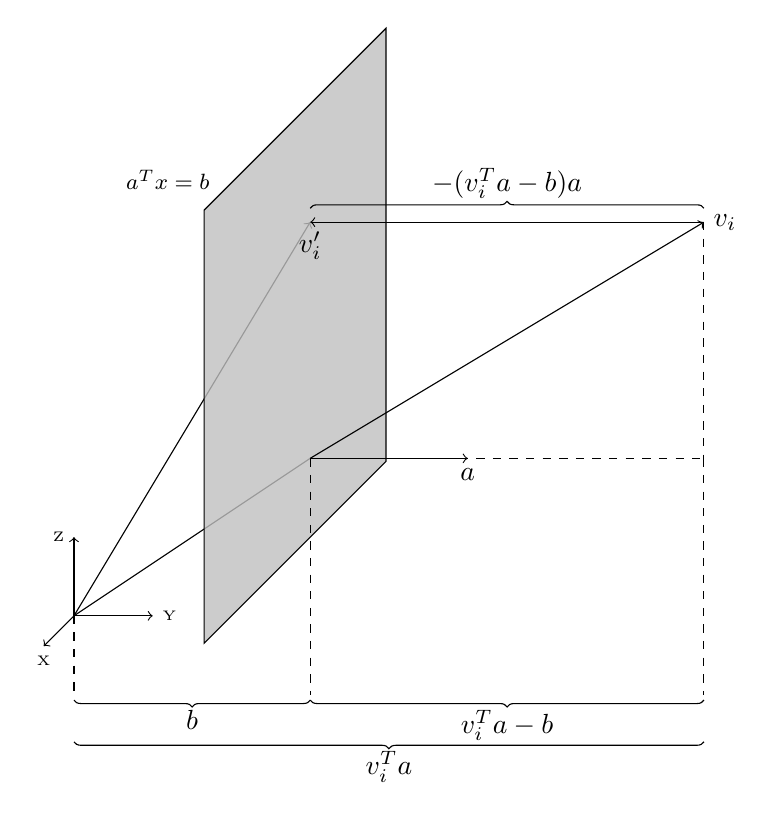
\begin{tikzpicture}[xyz frame={(0,0,-1)}{(0,1,0)}{(1,0,0)}]
\def\endZ{8}
\def\lowY{-1}
%%%axes
\draw[->] (0,0,0) -- (0,0,1)node[right,font=\tiny] {Y};
\draw[->] (0,0,0) -- (0,1,0)node[left,font=\tiny] {Z};
\draw[->] (0,0,0) -- (-1,0,0)node[below, font=\tiny] {X};
%%%hyperplane
\draw (-2.5,6.5,1.5)node[right, font=\footnotesize] {$a^Tx=b$};
\filldraw[fill=lightgray,fill opacity=0.8] (2.5,1,3) -- (2.5,6.5,3) --  (-3.5,6.5,3) -- (-3.5,1,3) -- cycle;

%%% v_i
\draw[on layer=behind] (0,0,0) -- (0,2,3);
\draw[on layer=in front, ->]  (0,2,3) -- (0,5,\endZ) node[right] {$v_i$};

%%% normal a
\draw[->]  (0,2,3) -- (0,2,5) node[below]{$a$};

%% v_i'
\draw[on layer=behind, -> ]  (0,0,0) -- (0,5,3);
\draw[<-]  (0,5,3)node[below]{$v_i'$} -- (0,5,\endZ);
\draw[decoration={brace},decorate,yshift=5pt]  (0,5,3) -- (0,5,\endZ)node[pos=0.5,above]{$-(v_i^Ta-b)a$};

%% plane to projection
\draw[-,dashed]  (0,2,3) -- (0,2,\endZ);
%% projection to v_i
\draw[-,dashed]  (0,5,\endZ) -- (0,2,\endZ);

%% lower annotations
\draw[-,dashed]  (0,0,0) -- (0,\lowY,0);
\draw[decoration={brace,mirror},decorate,yshift=-2pt]  (0,\lowY,0) -- (0,\lowY,3) node[pos=0.5,below]{$b$};
\draw[-,dashed]  (0,2,3) -- (0,\lowY,3);
\draw[decoration={brace,mirror},decorate,yshift=-0.6cm]  (0,\lowY,0) -- (0,\lowY,\endZ) node[pos=0.5,below]{$v_i^Ta$};
\draw[decoration={brace,mirror},decorate,yshift=-2pt]  (0,\lowY,3) -- (0,\lowY,\endZ) node[pos=0.5,below]{$v_i^Ta-b$};
\draw[-,dashed]  (0,2,\endZ) -- (0,\lowY,\endZ);

\end{tikzpicture}
\caption{Geometrical visualization that the orthogonal projection of a point
$v_i$ onto a hyperplane defined by $a^Tx=b$ is given by $v_i' = v_i -
(v_i^Ta-b)a$.\label{fig}}

\end{figure}

\section{Projection along line $L$}

Let $L=\{x \in \R^N| x = c + \lambda (d-c)\}$ be a line through point $c,d \in
\R^N$. Let $H=\{x\in \R^N| a^Tx=b\}$ be the hyperplane. The intersection of $L$
and $H$ is given by
\begin{equation}
        \begin{aligned}
                a^T(c+\lambda(d-c)) &= b\\
                   \lambda a^T(d-c) &= b - a^Tc\\
                            \lambda &= \frac{b-a^Tc}{a^T(d-c)} &|a^T(d-c)\neq 0
        \end{aligned}
\end{equation}
Thus, the intersection of $L$ and $H$ is given by the point 

\begin{equation}
        \begin{aligned}
                x_{LH} = c + \frac{b-a^Tc}{a^T(d-c)} (d-c)
        \end{aligned}
\end{equation}
for the case that $a^T(d-c)\neq 0$. If
$a^T(d-c)=0$, then the line is perpendicular to the plane normal, and thus
parallel to the plane, i.e. either it does not intersect the plane, or it lies
inside the hyperplane.

\section{Special Case: Projection of a point $v \in \R^3$ along line parallel to
z-axis}
Let $v \in \R^3$ be given. 
\begin{center}
     $L=\{x \in \R^3| x = v - \lambda (0,0,1)^T\}$\\
        $H=\{x\in \R^N| a^Tx=b\}$
\end{center}
Assume that $v \not\in H$, and $a^T(0,0,1)^T \neq 0$. Then $\lambda =
\frac{b-a^Tv}{a^T(0,0,1)^T}$. And the projection of $v$ onto $H$ along $L$ is
given by
\begin{center}
        $v' = v - \frac{b-a^Tv}{a^T(0,0,1)^T}(0,0,1)^T$
\end{center}


\end{document}
